% Asset ID: AS2MeasuresLocationSpreadTikZ-003
% Purpose: Show true class limits.
\documentclass[tikz,border=8pt]{standalone}
\usepackage{amsmath}
\usetikzlibrary{arrows.meta, positioning, decorations.pathreplacing}
\begin{document}
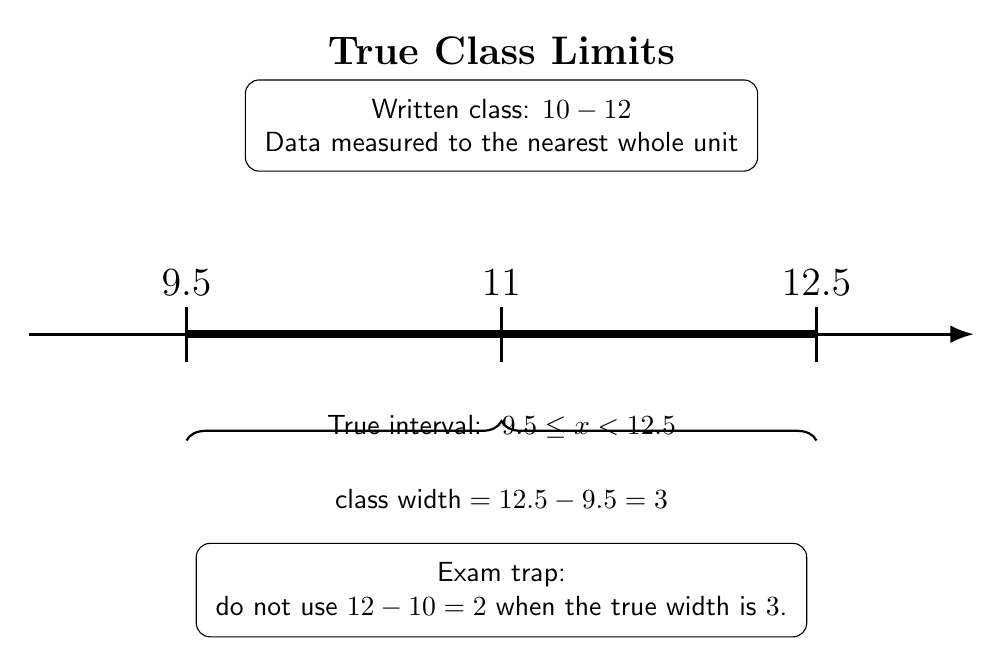
\begin{tikzpicture}[font=\sffamily, note/.style={draw, rounded corners=5pt, align=center, inner sep=7pt}, tick/.style={line width=1pt}]
\node[font=\Large\bfseries] at (0,4.4) {True Class Limits};
\node[note] at (0,3.45) {Written class: $10-12$\\Data measured to the nearest whole unit};
\draw[-{Latex[length=3mm]}, line width=1pt] (-6,0.8) -- (6,0.8);
\foreach \x/\lab in {-4/9.5,0/11,4/12.5}{\draw[tick] (\x,0.45) -- (\x,1.15);\node[font=\Large] at (\x,1.45) {$\lab$};}
\draw[line width=3pt] (-4,0.8) -- (4,0.8);
\node[below=9mm, align=center] at (0,0.8) {True interval: $\;9.5 \leq x < 12.5$};
\draw[decorate, decoration={brace, amplitude=7pt}, thick] (-4,-0.55) -- (4,-0.55);
\node[below=5mm] at (0,-0.55) {$\text{class width}=12.5-9.5=3$};
\node[note] at (0,-2.45) {Exam trap:\\do not use $12-10=2$ when the true width is $3$.};
\end{tikzpicture}
\end{document}
